\newpage
\chapter{Testing the parameterizations with existing data}
\mbox{}\vspace{-\baselineskip}





The Bosted parameterization~\cite{Bosted_fit,Bosted:2007xd} and the approximations of the peak cross section~\cite{Durand:1961zz,Kocevar:1967} were tested on two sets of published data, i.e. the first set consists of six measurements obtained for beam energies from 0.5 to 1.6~GeV and $Q^{2}$ from 0.3 to 1.8~GeV$^2$~\cite{Hanson:1973vf}, while the second set includes two measurements obtained for beam energies of 9.8 and 12.6~GeV and $Q^{2}$ of 2.5 and 4~GeV$^2$, respectively~\cite{Rock:1991jy,Rock_SLAC}\footnote[5]{Actually, the second set~\cite{Rock:1991jy,Rock_SLAC} contains three more measurements at $Q^{2} = $ 6, 8, and 10~GeV$^2$, but they are not considered here because the quasi-elastic peak vanishes for such high $Q^2$ values.}. %The former set is especially important, since its $Q^{2}$ coverage overlaps with that of this analysis. The latter set is used as a complimentary one.

Figure~\ref{fig:hanson_QE} shows the quasi-elastic peak for the first set of measurements~\cite{Hanson:1973vf} (black points) compared with the Bosted parameterization shown as histograms. The blue histograms correspond to the default way of $F^{QE}$ calculation (using the Paris wave function), while the green histograms correspond to $F^{QE}$ calculated by the alternative way (according to Eq.~\eqref{eq:fqe_scaling}). As is seen from Fig.~\ref{fig:hanson_QE}, although describing rather nicely the left and right distribution slopes, the blue histograms systematically overestimate the peak values. Meanwhile, the green histograms have worse description of the left slope and have a tendency to underestimate the peak cross sections. The parameterization histograms were produced together with the inelastic part of the spectrum to facilitate visual comparison with the experimental measurements and to account for inelastic background under the quasi-elastic peak. The green horizontal lines in Fig.~\ref{fig:hanson_QE} correspond to the peak cross section values approximated by Eq.~\eqref{eq:durand}, while the red lines correspond to the predictions of Eq.~(50) from Ref.~\cite{Kocevar:1967}. As is seen, the former describe nicely the experimental peak values, while the latter match well the maxima of the blue histograms of the Bosted parameterization.

\begin{figure}[htp]
\begin{center}
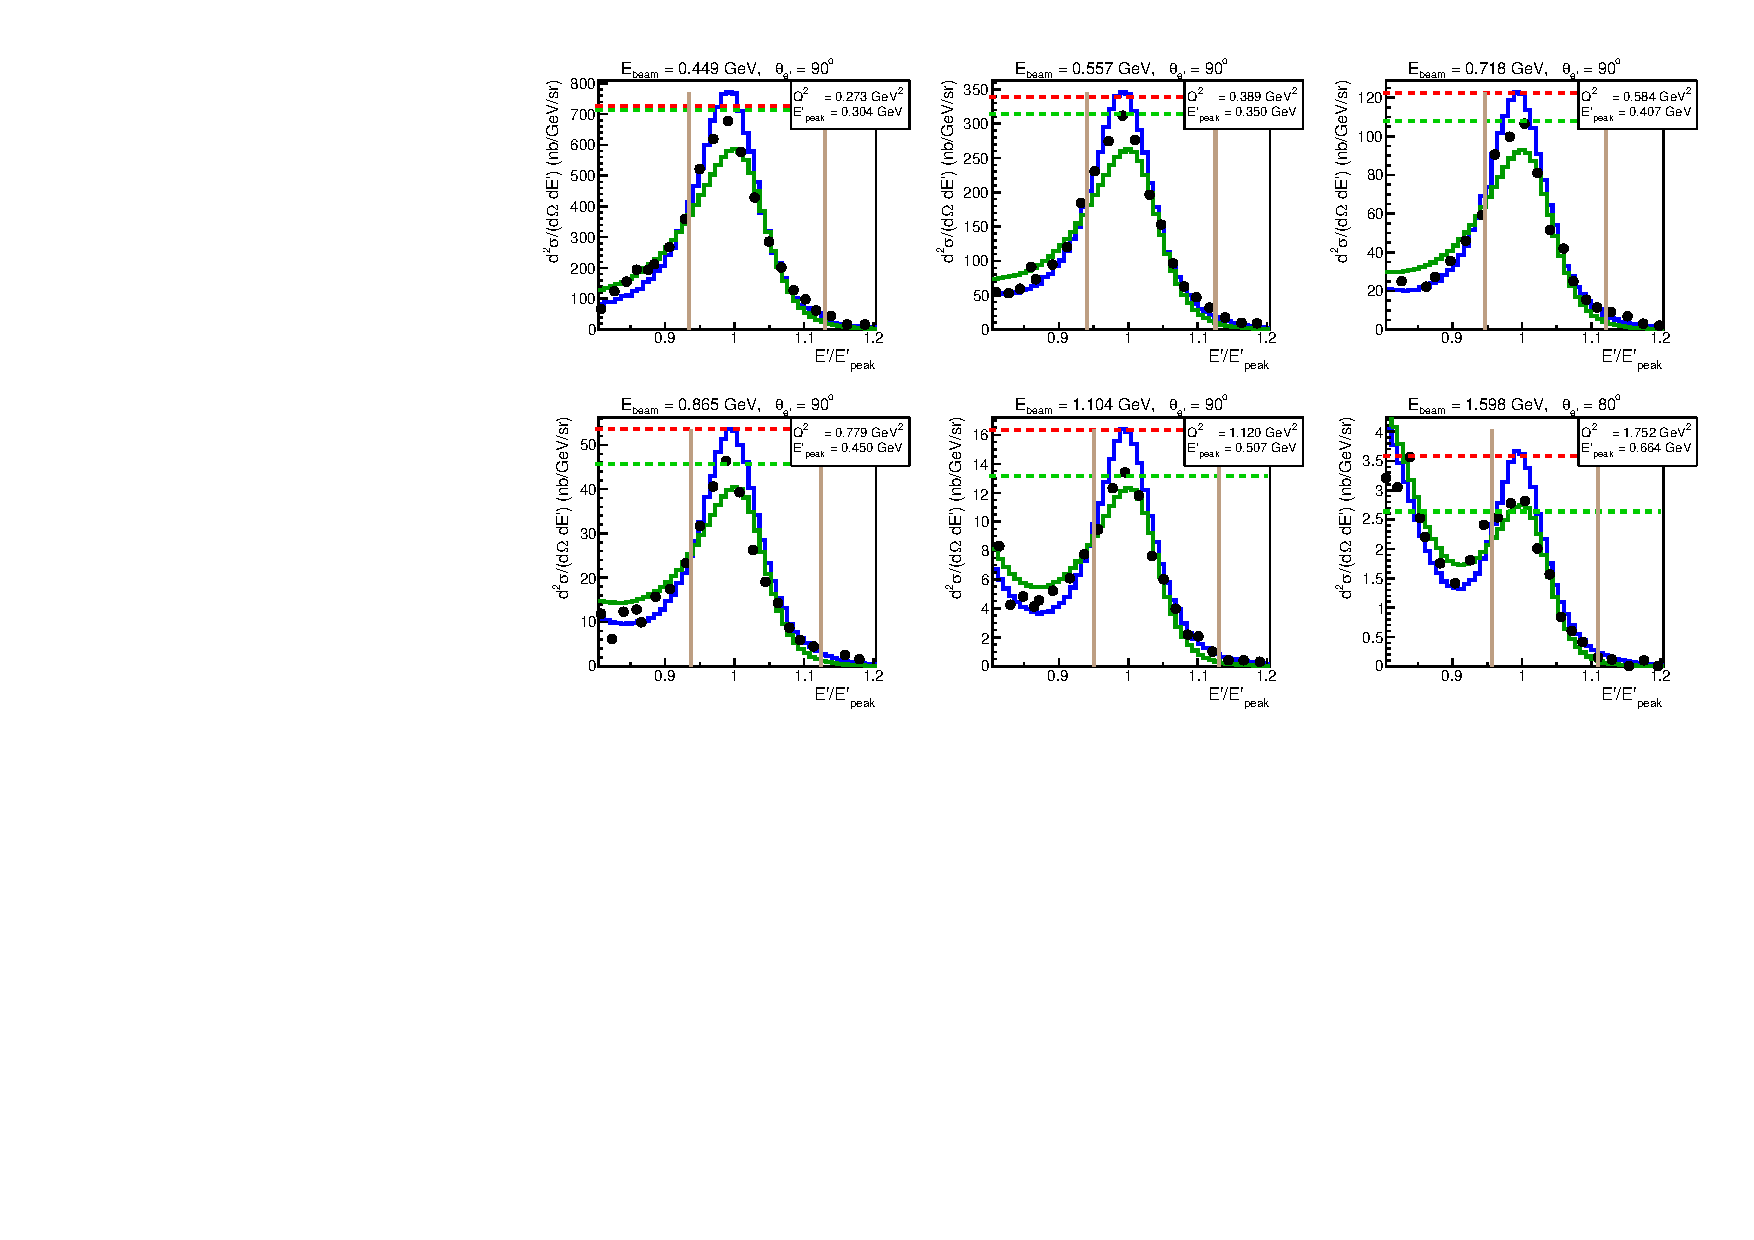
\includegraphics[width=\textwidth]{pictures/hanson.pdf}
\caption{\small  Data from Ref.~\cite{Hanson:1973vf} (black points) are compared with the Bosted parameterization~\cite{Bosted_fit,Bosted:2007xd} (histograms). The data uncertainties, which are on a level of 5\%, are not shown, see Ref.~\cite{Hanson:1973vf} on this matter. The blue histograms correspond to the default way of $F^{QE}$ calculation (using the Paris wave function), while the green ones correspond to $F^{QE}$ calculated by the alternative way (according to Eq.~\eqref{eq:fqe_scaling}). The green horizontal lines show the peak cross section values approximated by Eq.~\eqref{eq:durand}, while the red lines correspond to the predictions of Eq.~(50) from Ref.~\cite{Kocevar:1967}. The vertical lines show the integration limits.} \label{fig:hanson_QE}
\end{center}
\end{figure}


\afterpage{\clearpage}
\begin{figure}[htp]
\begin{center}
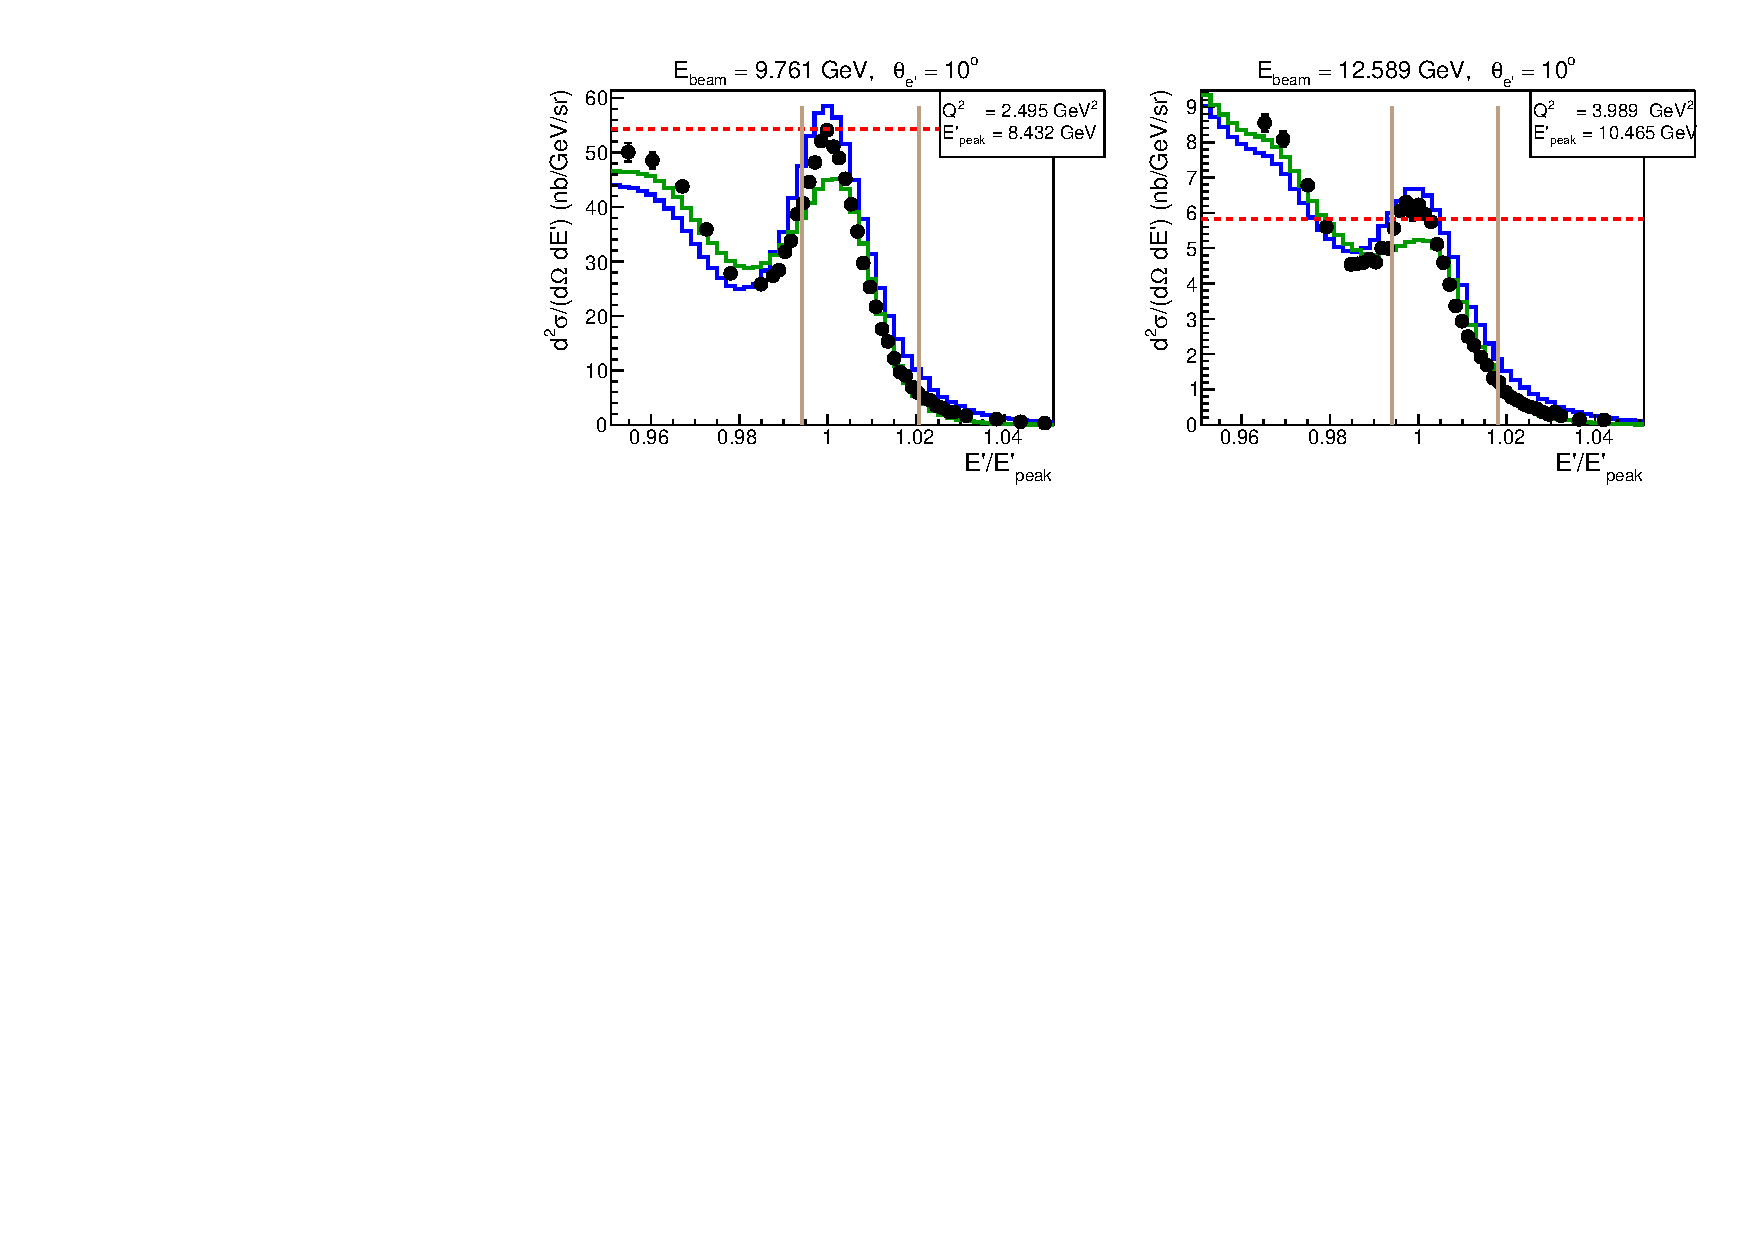
\includegraphics[width=14cm]{pictures/rock.pdf}
\caption{\small Data from Refs.~\cite{Rock:1991jy,Rock_SLAC} (black points) are compared with the Bosted parameterization~\cite{Bosted_fit,Bosted:2007xd} (histograms). The blue histograms correspond to the default way of $F^{QE}$ calculation (using the Paris wave function), while the green histograms correspond to $F^{QE}$ calculated by the alternative way (according to Eq.~\eqref{eq:fqe_scaling}). The red horizontal lines show the peak values predicted by Eq.~(50) from Ref.~\cite{Kocevar:1967}. The vertical lines show the integration limits.  } \label{fig:rock_QE}
\end{center}
\end{figure}
\begin{table}[htp]
\begin{center}
\caption{\small Ratios of the experimental integrals under the quasi-elastic peak ($\sigma_{exp}$) to those obtained from the Bosted parameterization~\cite{Bosted_fit,Bosted:2007xd}, in which $F^{QE}$ is calculated by using the Paris wave function ($\sigma_{par}^{1}$) or given by Eq.~\eqref{eq:fqe_scaling} ($\sigma_{par}^{2}$). The first six rows correspond to the first dataset from Ref.~\cite{Hanson:1973vf} and the last two to the second dataset from  Refs.~\cite{Rock:1991jy,Rock_SLAC}. The index $norm$ means that the parameterization histograms were scaled in a way that their maxima were equal to the predictions of Eq.~\eqref{eq:durand} for the first dataset and to the predictions of Eq.~(50) from Ref.~\cite{Kocevar:1967} for the second dataset. The coloring of the table cells is related to the corresponding deviation of the obtained ratio from unity: the dark-green shade stands for deviations $\leq 5$\%, light-green for 5\%-10\%, and light-red for more than 10\%.  \label{tab:quasi_el_tab}}
\begin{tabular}{
   !{\vrule width 2pt}
  c!{\vrule width 1pt}
  c!{\vrule width 1pt}
  c!{\vrule width 1pt}
  c!{\vrule width 2pt}
  c!{\vrule width 1pt}
  c!{\vrule width 2pt}
  c!{\vrule width 1pt}
  c!{\vrule width 2pt}
  }
\toprule[2pt]
\makecell{Exp.\\ Ref.} &\makecell{$E_{beam}$\\ (GeV)} &\makecell{$Q^{2}$\\ (GeV$^2$)} & \makecell{$E'_{peak}$ \\(GeV)} &$\sigma_{exp}/\sigma_{par}^{1}$ &$\sigma_{exp}/\sigma_{\substack{par, \\ norm}}^{1}$& $\sigma_{exp}/\sigma_{par}^{2}$ &$\sigma_{exp}/\sigma_{\substack{par, \\ norm}}^{2}$ \\ \hline
\multirow{6}{*}{\cite{Hanson:1973vf}}&0.449  &0.273  &0.304  &\cellcolor{green!20}0.94   &\cellcolor{green!35}1.02   &\cellcolor{red!20}1.14    &\cellcolor{green!20}0.93\\ \hhline{|~|-------|}
&0.557  &0.389  &0.350  &\cellcolor{green!20}0.93   &\cellcolor{green!35}1.03     &\cellcolor{red!20}1.14    &\cellcolor{green!35}0.95\\ \hhline{|~|-------|}
&0.718  &0.584  &0.407  &\cellcolor{green!20}0.91     &\cellcolor{green!35}1.03   &\cellcolor{red!20}1.12  &\cellcolor{green!35}0.96\\ \hhline{|~|-------|}
&0.865  &0.779  &0.450  &\cellcolor{red!20}0.84     &\cellcolor{green!35}0.99   &\cellcolor{green!35}1.04  &\cellcolor{green!20}0.92\\ \hhline{|~|-------|}
&1.104  &1.120  &0.507  &\cellcolor{red!20}0.85     &\cellcolor{green!35}1.05   &\cellcolor{green!20}1.06  &\cellcolor{green!35}1.00\\ \hhline{|~|-------|}
\multirow{5}{*}{\cite{Rock:1991jy,Rock_SLAC}}&1.598  &1.752  &0.664  &\cellcolor{red!20}0.85     &\cellcolor{red!20}1.18   &\cellcolor{green!20}1.06  &\cellcolor{red!20}1.11\\ \midrule[2pt]
&9.761  &2.495  &8.432  &\cellcolor{red!20}0.83     &\cellcolor{green!20}0.90     &\cellcolor{green!35}1.05  &\cellcolor{red!20}0.87\\ \hhline{|~|-------|}
&12.589 &3.989  &10.465 &\cellcolor{red!20}0.84     &\cellcolor{green!35}0.97     &\cellcolor{green!35}1.04  &\cellcolor{green!20}0.93\\ \bottomrule[2pt]
\end{tabular}
\end{center}
\end{table}

Figure~\ref{fig:rock_QE} shows the quasi-elastic peak for the second set of measurements~\cite{Rock:1991jy,Rock_SLAC} (black points) compared with the Bosted parameterization shown as histograms. Again, the blue histograms correspond to the default way of $F^{QE}$ calculation (using the Paris wave function), while the green ones correspond to $F^{QE}$ calculated by the alternative way (according to Eq.~\eqref{eq:fqe_scaling}). Here, the former systematically overestimate the experimental cross section for almost all data points, while the latter, although describing the slopes fairly well, underestimate the peak cross section. The red lines mark the peak cross section values given by Eq.~(50) from Ref.~\cite{Kocevar:1967}, which reasonably match the experiment. The peak values given by Eq.~\eqref{eq:durand} are not shown here, since this approximation does not work well for those high values of $Q^{2}$.

To estimate more quantitatively the overall quality of the data description by the Bosted parameterization, a comparison of the corresponding integrals under the quasi-elastic peak was performed. For this purpose all distributions were integrated within the limits shown by the vertical lines in Figs.~\ref{fig:hanson_QE} and~\ref{fig:rock_QE}. To determine the positions of these limits, the quasi-elastic peaks in the experimental spectra were fit by Gaussians with polynomial background. Then the values $\mu-\sigma$ and $\mu+3\sigma$ were set as the left and right integration limits, respectively, with $\mu$ and $\sigma$ being the mean value and the standard deviation of the corresponding Gaussian function. The integration limits were chosen to be asymmetrical in order to minimize the inelastic background under the quasi-elastic peak. This procedure of obtaining the integration limits was used in order to achieve consistency among all plots, since the width of the quasi-elastic peak and its proximity to the inelastic part of the spectrum depend on the kinematics.



The results of the performed comparison are summarized in Tab.~\ref{tab:quasi_el_tab}, where the first six rows correspond to the first dataset from Ref.~\cite{Hanson:1973vf}, while the last two correspond to the second dataset from  Refs.~\cite{Rock:1991jy,Rock_SLAC}. The last four columns contain the values of the ratio of the experimental integral under the quasi-elastic peak ($\sigma_{exp}$) to that obtained from the Bosted parameterization, in which $F^{QE}$ is calculated by using the Paris wave function ($\sigma_{par}^{1}$) or given by Eq.~\eqref{eq:fqe_scaling} ($\sigma_{par}^{2}$). The index $norm$ indicates that the parameterization histograms were scaled in a way that their maxima were equal to the predictions of Eq.~\eqref{eq:durand} for the first dataset and to the predictions of Eq.~(50) from Ref.~\cite{Kocevar:1967} for the second dataset. The coloring of the table cells is related to the corresponding deviation of the obtained ratio from unity\footnote[6]{The ratio values given in Tab.~\ref{tab:quasi_el_tab} are slightly dependent on the positions of the integration limits, but the overall behavior of the data description quality reflected in the table is stable.}: the dark-green shade stands for deviations $\leq 5$\%, light-green for 5\%-10\%, and light-red for more than 10\%. 

%{Although the ratio values given in Tab.~\ref{tab:quasi_el_tab} have some dependence on the position of the integration limits, the overall behavior of the data description reflected in the table is rather stable.
As is seen from Tab.~\ref{tab:quasi_el_tab}, the Bosted parameterization with $F_{QE}$ calculated by the default method systematically overestimates the measured integral cross sections under the quasi-elastic peak, while with $F_{QE}$ calculated in the alternative way it systematically underestimates them. Beside this, when normalized to the values provided by the corresponding peak cross section approximations~\cite{Durand:1961zz,Kocevar:1967}, the Bosted parameterization better describes the integral cross sections for the majority of considered measurements.



